\subsubsection{Acondicionamiento de señales $M_{22}$}

Debido a cómo están configurados los sensores seleccionados, el proceso de acondicionamiento de la señal se realiza de forma digital al interior de la tarjeta de desarrollo a través de las librerías que existen en el entorno de desarrollo, por lo que el circuito electrónico es mas simple, solo se utilizaron unas cuantas resistencias, sugeridas por los proveedores que están conectadas entre la salida de datos del sensor y el pin donde estarán conectados a la tarjeta de desarrollo.

Esto se hizo con el fin de reducir las interferencias de ruido, además de provocar una caída de tensión para la lectura de los pulsos digitales. La forma en como se puede realizar su conexión en una tarjeta de desarrollo se puede ver en las figuras \ref{fg:tempacpnd} y \ref{fg:dht11acondi}

Finalmente, los sensores se integraron al esquema que se realizo para la interfaz, donde están conectados a la tarjeta ESP-32 como se muestra en la figura \ref{fg:CTO MONITOREO}



\begin{figure}[h!]
            \centering
            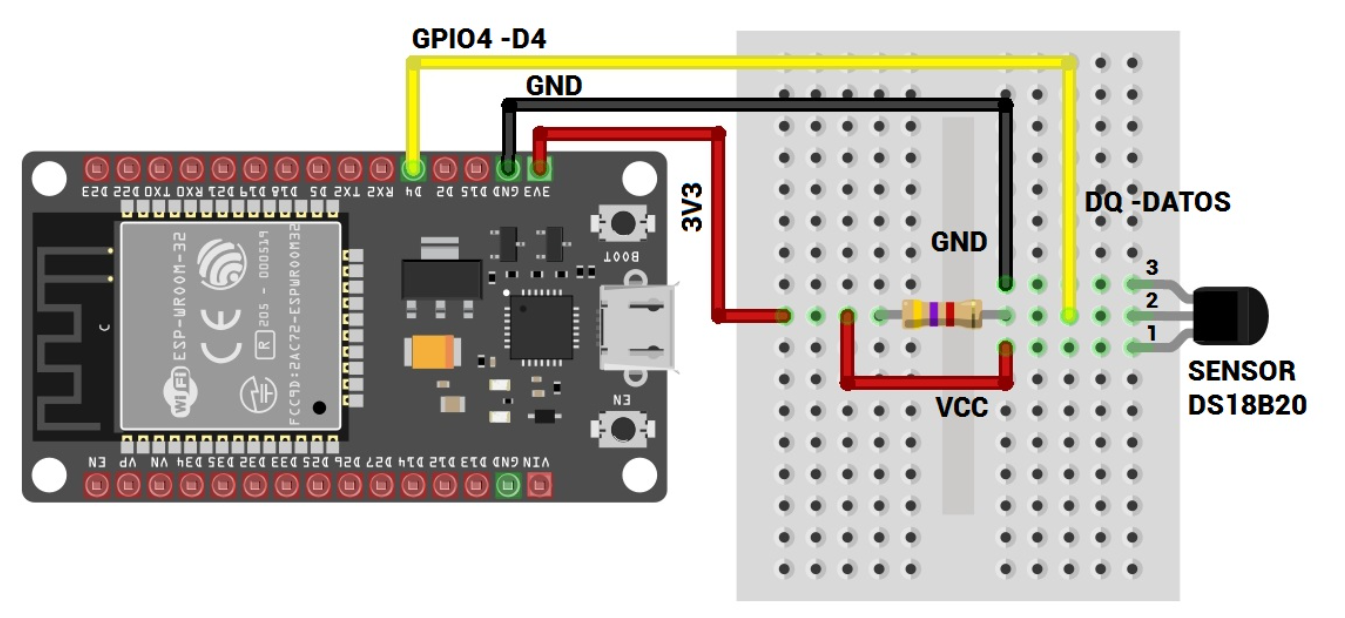
\includegraphics[scale=0.25]{images/Capitulo 4/S2/tempacons.png}
            \caption{Ejemplo de conexión del sensor DS18B20 a una tarjeta de desarrollo \cite{TempSensor}}
            \label{fg:tempacpnd}
        \end{figure}

\begin{figure}[h!]
            \centering
            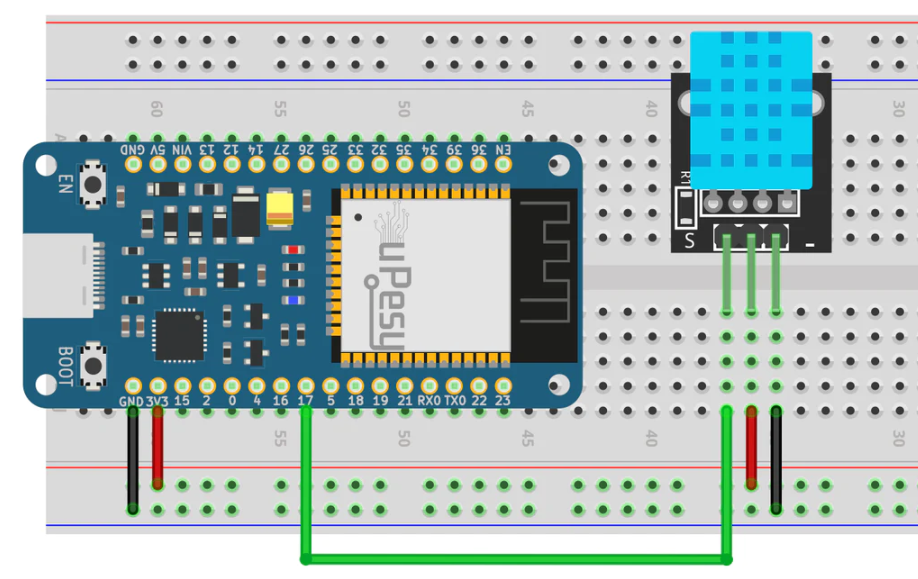
\includegraphics[scale=0.25]{images/Capitulo 4/S2/DHT11ACON.png}
            \caption{Ejemplo de conexión del sensor de humedad DHT11 a una tarjeta de desarrollo \cite{DHT11acon}}
            \label{fg:dht11acondi}
        \end{figure}

\begin{figure}[h!]
            \centering
            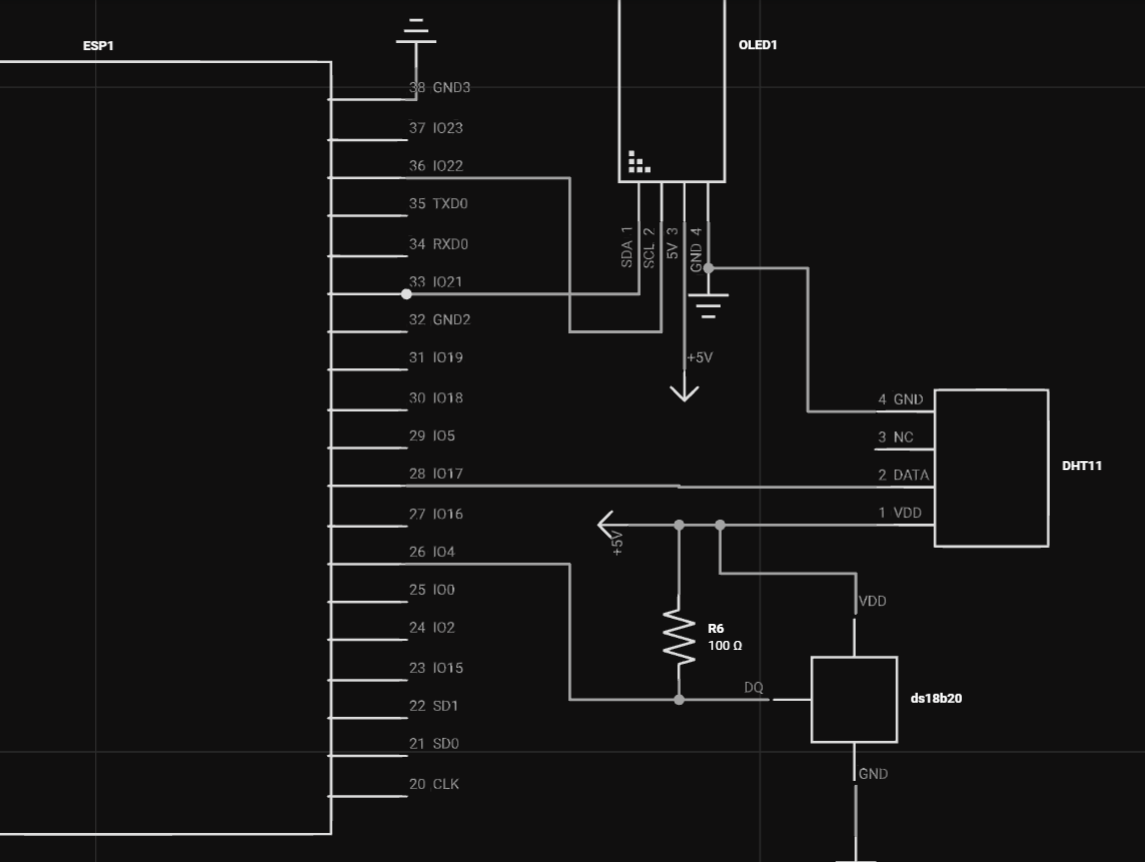
\includegraphics[scale=0.25]{images/Capitulo 4/S2/CTO Monitoreo.png}
            \caption{Integración de los sensores en la tarjeta de desarrollo}
            \label{fg:CTO MONITOREO}
        \end{figure}


\newpage
